% Created by tikzDevice version 0.12 on 2019-04-23 13:46:35
% !TEX encoding = UTF-8 Unicode
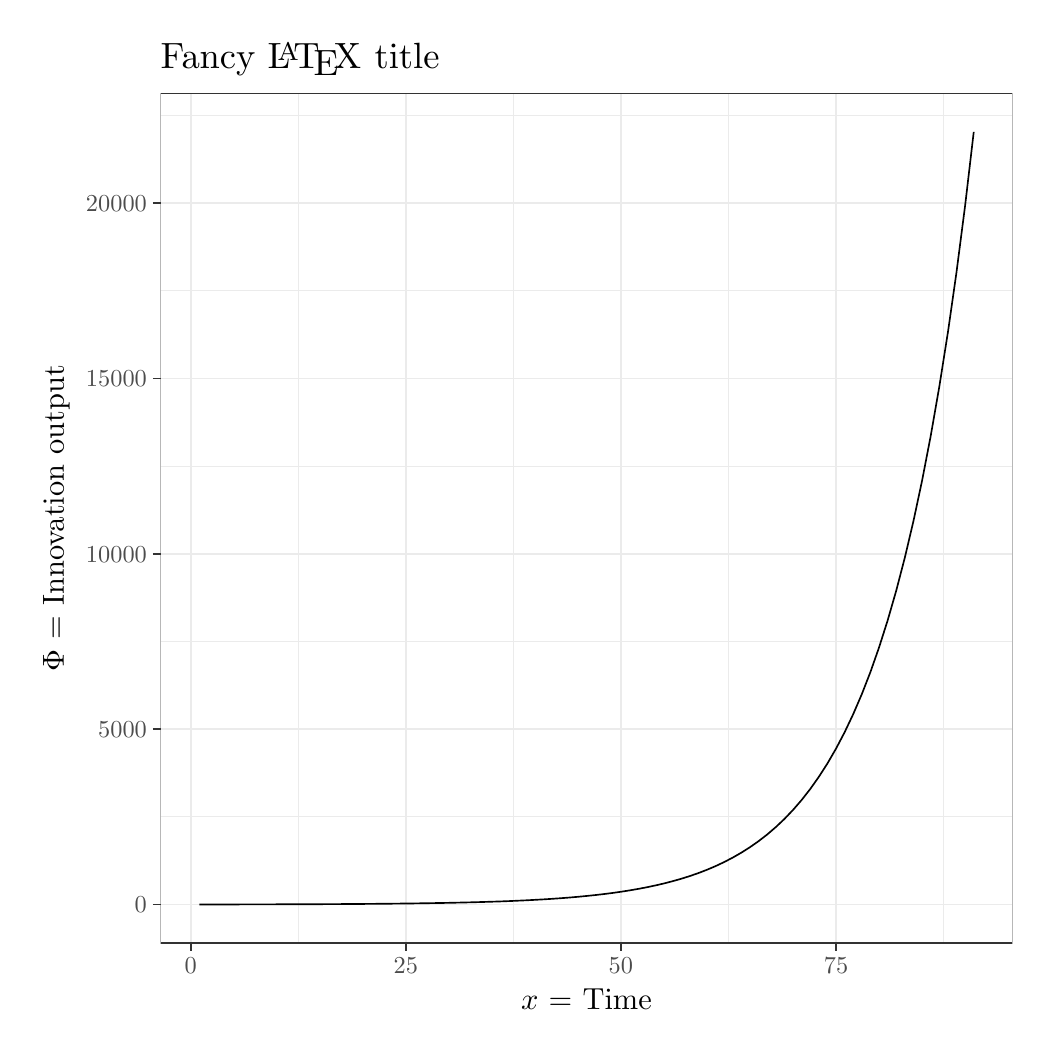
\begin{tikzpicture}[x=1pt,y=1pt]
\definecolor{fillColor}{RGB}{255,255,255}
\path[use as bounding box,fill=fillColor,fill opacity=0.00] (0,0) rectangle (361.35,361.35);
\begin{scope}
\path[clip] (  0.00,  0.00) rectangle (361.35,361.35);
\definecolor{drawColor}{RGB}{255,255,255}
\definecolor{fillColor}{RGB}{255,255,255}

\path[draw=drawColor,line width= 0.6pt,line join=round,line cap=round,fill=fillColor] (  0.00,  0.00) rectangle (361.35,361.35);
\end{scope}
\begin{scope}
\path[clip] ( 48.02, 30.56) rectangle (355.85,337.66);
\definecolor{fillColor}{RGB}{255,255,255}

\path[fill=fillColor] ( 48.02, 30.56) rectangle (355.85,337.66);
\definecolor{drawColor}{gray}{0.92}

\path[draw=drawColor,line width= 0.3pt,line join=round] ( 48.02, 76.17) --
	(355.85, 76.17);

\path[draw=drawColor,line width= 0.3pt,line join=round] ( 48.02,139.56) --
	(355.85,139.56);

\path[draw=drawColor,line width= 0.3pt,line join=round] ( 48.02,202.94) --
	(355.85,202.94);

\path[draw=drawColor,line width= 0.3pt,line join=round] ( 48.02,266.32) --
	(355.85,266.32);

\path[draw=drawColor,line width= 0.3pt,line join=round] ( 48.02,329.70) --
	(355.85,329.70);

\path[draw=drawColor,line width= 0.3pt,line join=round] ( 97.77, 30.56) --
	( 97.77,337.66);

\path[draw=drawColor,line width= 0.3pt,line join=round] (175.51, 30.56) --
	(175.51,337.66);

\path[draw=drawColor,line width= 0.3pt,line join=round] (253.24, 30.56) --
	(253.24,337.66);

\path[draw=drawColor,line width= 0.3pt,line join=round] (330.97, 30.56) --
	(330.97,337.66);

\path[draw=drawColor,line width= 0.6pt,line join=round] ( 48.02, 44.48) --
	(355.85, 44.48);

\path[draw=drawColor,line width= 0.6pt,line join=round] ( 48.02,107.87) --
	(355.85,107.87);

\path[draw=drawColor,line width= 0.6pt,line join=round] ( 48.02,171.25) --
	(355.85,171.25);

\path[draw=drawColor,line width= 0.6pt,line join=round] ( 48.02,234.63) --
	(355.85,234.63);

\path[draw=drawColor,line width= 0.6pt,line join=round] ( 48.02,298.01) --
	(355.85,298.01);

\path[draw=drawColor,line width= 0.6pt,line join=round] ( 58.90, 30.56) --
	( 58.90,337.66);

\path[draw=drawColor,line width= 0.6pt,line join=round] (136.64, 30.56) --
	(136.64,337.66);

\path[draw=drawColor,line width= 0.6pt,line join=round] (214.37, 30.56) --
	(214.37,337.66);

\path[draw=drawColor,line width= 0.6pt,line join=round] (292.11, 30.56) --
	(292.11,337.66);
\definecolor{drawColor}{RGB}{0,0,0}

\path[draw=drawColor,line width= 0.6pt,line join=round] ( 62.01, 44.52) --
	( 65.12, 44.52) --
	( 68.23, 44.53) --
	( 71.34, 44.53) --
	( 74.45, 44.53) --
	( 77.56, 44.54) --
	( 80.67, 44.55) --
	( 83.78, 44.55) --
	( 86.89, 44.56) --
	( 90.00, 44.57) --
	( 93.11, 44.58) --
	( 96.22, 44.59) --
	( 99.33, 44.60) --
	(102.43, 44.61) --
	(105.54, 44.62) --
	(108.65, 44.64) --
	(111.76, 44.65) --
	(114.87, 44.67) --
	(117.98, 44.69) --
	(121.09, 44.71) --
	(124.20, 44.74) --
	(127.31, 44.76) --
	(130.42, 44.79) --
	(133.53, 44.83) --
	(136.64, 44.86) --
	(139.75, 44.90) --
	(142.86, 44.95) --
	(145.97, 45.00) --
	(149.08, 45.05) --
	(152.18, 45.11) --
	(155.29, 45.18) --
	(158.40, 45.25) --
	(161.51, 45.33) --
	(164.62, 45.42) --
	(167.73, 45.52) --
	(170.84, 45.62) --
	(173.95, 45.74) --
	(177.06, 45.88) --
	(180.17, 46.02) --
	(183.28, 46.19) --
	(186.39, 46.36) --
	(189.50, 46.56) --
	(192.61, 46.78) --
	(195.72, 47.02) --
	(198.83, 47.29) --
	(201.94, 47.59) --
	(205.04, 47.91) --
	(208.15, 48.27) --
	(211.26, 48.67) --
	(214.37, 49.11) --
	(217.48, 49.60) --
	(220.59, 50.14) --
	(223.70, 50.73) --
	(226.81, 51.39) --
	(229.92, 52.11) --
	(233.03, 52.92) --
	(236.14, 53.80) --
	(239.25, 54.78) --
	(242.36, 55.86) --
	(245.47, 57.06) --
	(248.58, 58.38) --
	(251.69, 59.85) --
	(254.79, 61.46) --
	(257.90, 63.25) --
	(261.01, 65.22) --
	(264.12, 67.40) --
	(267.23, 69.81) --
	(270.34, 72.48) --
	(273.45, 75.42) --
	(276.56, 78.68) --
	(279.67, 82.27) --
	(282.78, 86.25) --
	(285.89, 90.64) --
	(289.00, 95.49) --
	(292.11,100.86) --
	(295.22,106.79) --
	(298.33,113.34) --
	(301.44,120.58) --
	(304.55,128.58) --
	(307.65,137.43) --
	(310.76,147.20) --
	(313.87,158.00) --
	(316.98,169.94) --
	(320.09,183.14) --
	(323.20,197.72) --
	(326.31,213.84) --
	(329.42,231.65) --
	(332.53,251.33) --
	(335.64,273.09) --
	(338.75,297.13) --
	(341.86,323.70);
\definecolor{drawColor}{gray}{0.20}

\path[draw=drawColor,line width= 0.6pt,line join=round,line cap=round] ( 48.02, 30.56) rectangle (355.85,337.66);
\end{scope}
\begin{scope}
\path[clip] (  0.00,  0.00) rectangle (361.35,361.35);
\definecolor{drawColor}{gray}{0.30}

\node[text=drawColor,anchor=base east,inner sep=0pt, outer sep=0pt, scale=  0.88] at ( 43.07, 41.45) {0};

\node[text=drawColor,anchor=base east,inner sep=0pt, outer sep=0pt, scale=  0.88] at ( 43.07,104.84) {5000};

\node[text=drawColor,anchor=base east,inner sep=0pt, outer sep=0pt, scale=  0.88] at ( 43.07,168.22) {10000};

\node[text=drawColor,anchor=base east,inner sep=0pt, outer sep=0pt, scale=  0.88] at ( 43.07,231.60) {15000};

\node[text=drawColor,anchor=base east,inner sep=0pt, outer sep=0pt, scale=  0.88] at ( 43.07,294.98) {20000};
\end{scope}
\begin{scope}
\path[clip] (  0.00,  0.00) rectangle (361.35,361.35);
\definecolor{drawColor}{gray}{0.20}

\path[draw=drawColor,line width= 0.6pt,line join=round] ( 45.27, 44.48) --
	( 48.02, 44.48);

\path[draw=drawColor,line width= 0.6pt,line join=round] ( 45.27,107.87) --
	( 48.02,107.87);

\path[draw=drawColor,line width= 0.6pt,line join=round] ( 45.27,171.25) --
	( 48.02,171.25);

\path[draw=drawColor,line width= 0.6pt,line join=round] ( 45.27,234.63) --
	( 48.02,234.63);

\path[draw=drawColor,line width= 0.6pt,line join=round] ( 45.27,298.01) --
	( 48.02,298.01);
\end{scope}
\begin{scope}
\path[clip] (  0.00,  0.00) rectangle (361.35,361.35);
\definecolor{drawColor}{gray}{0.20}

\path[draw=drawColor,line width= 0.6pt,line join=round] ( 58.90, 27.81) --
	( 58.90, 30.56);

\path[draw=drawColor,line width= 0.6pt,line join=round] (136.64, 27.81) --
	(136.64, 30.56);

\path[draw=drawColor,line width= 0.6pt,line join=round] (214.37, 27.81) --
	(214.37, 30.56);

\path[draw=drawColor,line width= 0.6pt,line join=round] (292.11, 27.81) --
	(292.11, 30.56);
\end{scope}
\begin{scope}
\path[clip] (  0.00,  0.00) rectangle (361.35,361.35);
\definecolor{drawColor}{gray}{0.30}

\node[text=drawColor,anchor=base,inner sep=0pt, outer sep=0pt, scale=  0.88] at ( 58.90, 19.55) {0};

\node[text=drawColor,anchor=base,inner sep=0pt, outer sep=0pt, scale=  0.88] at (136.64, 19.55) {25};

\node[text=drawColor,anchor=base,inner sep=0pt, outer sep=0pt, scale=  0.88] at (214.37, 19.55) {50};

\node[text=drawColor,anchor=base,inner sep=0pt, outer sep=0pt, scale=  0.88] at (292.11, 19.55) {75};
\end{scope}
\begin{scope}
\path[clip] (  0.00,  0.00) rectangle (361.35,361.35);
\definecolor{drawColor}{RGB}{0,0,0}

\node[text=drawColor,anchor=base,inner sep=0pt, outer sep=0pt, scale=  1.10] at (201.94,  6.47) {$x$ = Time};
\end{scope}
\begin{scope}
\path[clip] (  0.00,  0.00) rectangle (361.35,361.35);
\definecolor{drawColor}{RGB}{0,0,0}

\node[text=drawColor,rotate= 90.00,anchor=base,inner sep=0pt, outer sep=0pt, scale=  1.10] at ( 13.08,184.11) {$\Phi$ = Innovation output};
\end{scope}
\begin{scope}
\path[clip] (  0.00,  0.00) rectangle (361.35,361.35);
\definecolor{drawColor}{RGB}{0,0,0}

\node[text=drawColor,anchor=base west,inner sep=0pt, outer sep=0pt, scale=  1.32] at ( 48.02,346.76) {Fancy \LaTeX  \hspace{0.01cm} title};
\end{scope}
\end{tikzpicture}
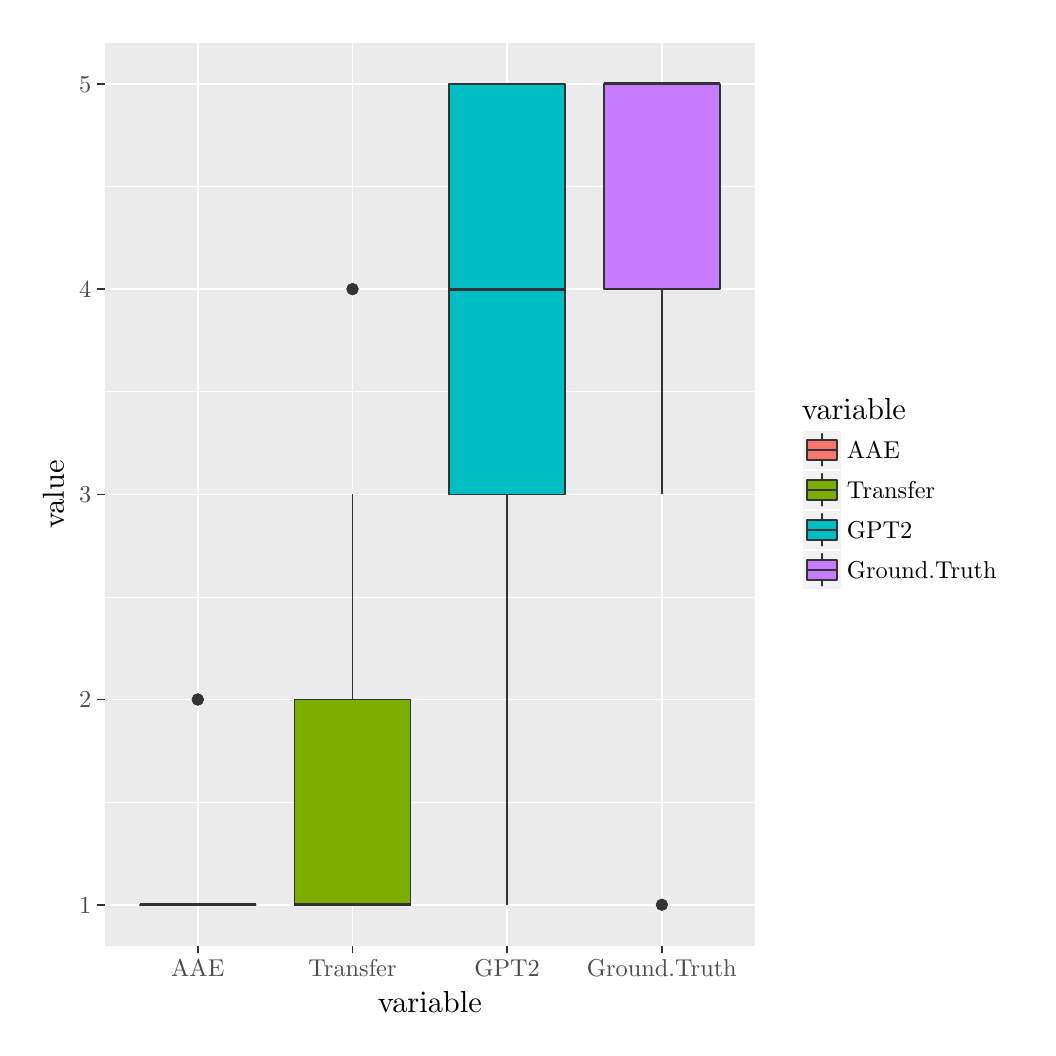
\begin{tikzpicture}[x=1pt,y=1pt]
\definecolor{fillColor}{RGB}{255,255,255}
\path[use as bounding box,fill=fillColor,fill opacity=0.00] (0,0) rectangle (361.35,361.35);
\begin{scope}
\path[clip] (  0.00,  0.00) rectangle (361.35,361.35);
\definecolor{drawColor}{RGB}{255,255,255}
\definecolor{fillColor}{RGB}{255,255,255}

\path[draw=drawColor,line width= 0.6pt,line join=round,line cap=round,fill=fillColor] (  0.00, -0.00) rectangle (361.35,361.35);
\end{scope}
\begin{scope}
\path[clip] ( 27.92, 29.59) rectangle (262.71,355.85);
\definecolor{fillColor}{gray}{0.92}

\path[fill=fillColor] ( 27.92, 29.59) rectangle (262.71,355.85);
\definecolor{drawColor}{RGB}{255,255,255}

\path[draw=drawColor,line width= 0.3pt,line join=round] ( 27.92, 81.49) --
	(262.71, 81.49);

\path[draw=drawColor,line width= 0.3pt,line join=round] ( 27.92,155.64) --
	(262.71,155.64);

\path[draw=drawColor,line width= 0.3pt,line join=round] ( 27.92,229.79) --
	(262.71,229.79);

\path[draw=drawColor,line width= 0.3pt,line join=round] ( 27.92,303.94) --
	(262.71,303.94);

\path[draw=drawColor,line width= 0.6pt,line join=round] ( 27.92, 44.42) --
	(262.71, 44.42);

\path[draw=drawColor,line width= 0.6pt,line join=round] ( 27.92,118.57) --
	(262.71,118.57);

\path[draw=drawColor,line width= 0.6pt,line join=round] ( 27.92,192.72) --
	(262.71,192.72);

\path[draw=drawColor,line width= 0.6pt,line join=round] ( 27.92,266.87) --
	(262.71,266.87);

\path[draw=drawColor,line width= 0.6pt,line join=round] ( 27.92,341.02) --
	(262.71,341.02);

\path[draw=drawColor,line width= 0.6pt,line join=round] ( 61.47, 29.59) --
	( 61.47,355.85);

\path[draw=drawColor,line width= 0.6pt,line join=round] (117.37, 29.59) --
	(117.37,355.85);

\path[draw=drawColor,line width= 0.6pt,line join=round] (173.27, 29.59) --
	(173.27,355.85);

\path[draw=drawColor,line width= 0.6pt,line join=round] (229.17, 29.59) --
	(229.17,355.85);
\definecolor{drawColor}{gray}{0.20}
\definecolor{fillColor}{gray}{0.20}

\path[draw=drawColor,line width= 0.4pt,line join=round,line cap=round,fill=fillColor] ( 61.47,118.57) circle (  1.96);

\path[draw=drawColor,line width= 0.4pt,line join=round,line cap=round,fill=fillColor] ( 61.47,118.57) circle (  1.96);

\path[draw=drawColor,line width= 0.4pt,line join=round,line cap=round,fill=fillColor] ( 61.47,118.57) circle (  1.96);

\path[draw=drawColor,line width= 0.4pt,line join=round,line cap=round,fill=fillColor] ( 61.47,118.57) circle (  1.96);

\path[draw=drawColor,line width= 0.6pt,line join=round] ( 61.47, 44.42) -- ( 61.47, 44.42);

\path[draw=drawColor,line width= 0.6pt,line join=round] ( 61.47, 44.42) -- ( 61.47, 44.42);
\definecolor{fillColor}{RGB}{248,118,109}

\path[draw=drawColor,line width= 0.6pt,line join=round,line cap=round,fill=fillColor] ( 40.50, 44.42) --
	( 40.50, 44.42) --
	( 82.43, 44.42) --
	( 82.43, 44.42) --
	( 40.50, 44.42) --
	cycle;

\path[draw=drawColor,line width= 1.1pt,line join=round] ( 40.50, 44.42) -- ( 82.43, 44.42);
\definecolor{fillColor}{gray}{0.20}

\path[draw=drawColor,line width= 0.4pt,line join=round,line cap=round,fill=fillColor] (117.37,266.87) circle (  1.96);

\path[draw=drawColor,line width= 0.4pt,line join=round,line cap=round,fill=fillColor] (117.37,266.87) circle (  1.96);

\path[draw=drawColor,line width= 0.4pt,line join=round,line cap=round,fill=fillColor] (117.37,266.87) circle (  1.96);

\path[draw=drawColor,line width= 0.6pt,line join=round] (117.37,118.57) -- (117.37,192.72);

\path[draw=drawColor,line width= 0.6pt,line join=round] (117.37, 44.42) -- (117.37, 44.42);
\definecolor{fillColor}{RGB}{124,174,0}

\path[draw=drawColor,line width= 0.6pt,line join=round,line cap=round,fill=fillColor] ( 96.40,118.57) --
	( 96.40, 44.42) --
	(138.33, 44.42) --
	(138.33,118.57) --
	( 96.40,118.57) --
	cycle;

\path[draw=drawColor,line width= 1.1pt,line join=round] ( 96.40, 44.42) -- (138.33, 44.42);

\path[draw=drawColor,line width= 0.6pt,line join=round] (173.27,341.02) -- (173.27,341.02);

\path[draw=drawColor,line width= 0.6pt,line join=round] (173.27,192.72) -- (173.27, 44.42);
\definecolor{fillColor}{RGB}{0,191,196}

\path[draw=drawColor,line width= 0.6pt,line join=round,line cap=round,fill=fillColor] (152.30,341.02) --
	(152.30,192.72) --
	(194.23,192.72) --
	(194.23,341.02) --
	(152.30,341.02) --
	cycle;

\path[draw=drawColor,line width= 1.1pt,line join=round] (152.30,266.87) -- (194.23,266.87);
\definecolor{fillColor}{gray}{0.20}

\path[draw=drawColor,line width= 0.4pt,line join=round,line cap=round,fill=fillColor] (229.17, 44.42) circle (  1.96);

\path[draw=drawColor,line width= 0.4pt,line join=round,line cap=round,fill=fillColor] (229.17, 44.42) circle (  1.96);

\path[draw=drawColor,line width= 0.6pt,line join=round] (229.17,341.02) -- (229.17,341.02);

\path[draw=drawColor,line width= 0.6pt,line join=round] (229.17,266.87) -- (229.17,192.72);
\definecolor{fillColor}{RGB}{199,124,255}

\path[draw=drawColor,line width= 0.6pt,line join=round,line cap=round,fill=fillColor] (208.20,341.02) --
	(208.20,266.87) --
	(250.13,266.87) --
	(250.13,341.02) --
	(208.20,341.02) --
	cycle;

\path[draw=drawColor,line width= 1.1pt,line join=round] (208.20,341.02) -- (250.13,341.02);
\end{scope}
\begin{scope}
\path[clip] (  0.00,  0.00) rectangle (361.35,361.35);
\definecolor{drawColor}{gray}{0.30}

\node[text=drawColor,anchor=base east,inner sep=0pt, outer sep=0pt, scale=  0.88] at ( 22.97, 41.39) {1};

\node[text=drawColor,anchor=base east,inner sep=0pt, outer sep=0pt, scale=  0.88] at ( 22.97,115.54) {2};

\node[text=drawColor,anchor=base east,inner sep=0pt, outer sep=0pt, scale=  0.88] at ( 22.97,189.69) {3};

\node[text=drawColor,anchor=base east,inner sep=0pt, outer sep=0pt, scale=  0.88] at ( 22.97,263.84) {4};

\node[text=drawColor,anchor=base east,inner sep=0pt, outer sep=0pt, scale=  0.88] at ( 22.97,337.99) {5};
\end{scope}
\begin{scope}
\path[clip] (  0.00,  0.00) rectangle (361.35,361.35);
\definecolor{drawColor}{gray}{0.20}

\path[draw=drawColor,line width= 0.6pt,line join=round] ( 25.17, 44.42) --
	( 27.92, 44.42);

\path[draw=drawColor,line width= 0.6pt,line join=round] ( 25.17,118.57) --
	( 27.92,118.57);

\path[draw=drawColor,line width= 0.6pt,line join=round] ( 25.17,192.72) --
	( 27.92,192.72);

\path[draw=drawColor,line width= 0.6pt,line join=round] ( 25.17,266.87) --
	( 27.92,266.87);

\path[draw=drawColor,line width= 0.6pt,line join=round] ( 25.17,341.02) --
	( 27.92,341.02);
\end{scope}
\begin{scope}
\path[clip] (  0.00,  0.00) rectangle (361.35,361.35);
\definecolor{drawColor}{gray}{0.20}

\path[draw=drawColor,line width= 0.6pt,line join=round] ( 61.47, 26.84) --
	( 61.47, 29.59);

\path[draw=drawColor,line width= 0.6pt,line join=round] (117.37, 26.84) --
	(117.37, 29.59);

\path[draw=drawColor,line width= 0.6pt,line join=round] (173.27, 26.84) --
	(173.27, 29.59);

\path[draw=drawColor,line width= 0.6pt,line join=round] (229.17, 26.84) --
	(229.17, 29.59);
\end{scope}
\begin{scope}
\path[clip] (  0.00,  0.00) rectangle (361.35,361.35);
\definecolor{drawColor}{gray}{0.30}

\node[text=drawColor,anchor=base,inner sep=0pt, outer sep=0pt, scale=  0.88] at ( 61.47, 18.58) {AAE};

\node[text=drawColor,anchor=base,inner sep=0pt, outer sep=0pt, scale=  0.88] at (117.37, 18.58) {Transfer};

\node[text=drawColor,anchor=base,inner sep=0pt, outer sep=0pt, scale=  0.88] at (173.27, 18.58) {GPT2};

\node[text=drawColor,anchor=base,inner sep=0pt, outer sep=0pt, scale=  0.88] at (229.17, 18.58) {Ground.Truth};
\end{scope}
\begin{scope}
\path[clip] (  0.00,  0.00) rectangle (361.35,361.35);
\definecolor{drawColor}{RGB}{0,0,0}

\node[text=drawColor,anchor=base,inner sep=0pt, outer sep=0pt, scale=  1.10] at (145.32,  5.50) {variable};
\end{scope}
\begin{scope}
\path[clip] (  0.00,  0.00) rectangle (361.35,361.35);
\definecolor{drawColor}{RGB}{0,0,0}

\node[text=drawColor,rotate= 90.00,anchor=base,inner sep=0pt, outer sep=0pt, scale=  1.10] at ( 13.08,192.72) {value};
\end{scope}
\begin{scope}
\path[clip] (  0.00,  0.00) rectangle (361.35,361.35);
\definecolor{fillColor}{RGB}{255,255,255}

\path[fill=fillColor] (274.09,152.53) rectangle (355.85,232.91);
\end{scope}
\begin{scope}
\path[clip] (  0.00,  0.00) rectangle (361.35,361.35);
\definecolor{drawColor}{RGB}{0,0,0}

\node[text=drawColor,anchor=base west,inner sep=0pt, outer sep=0pt, scale=  1.10] at (279.78,219.65) {variable};
\end{scope}
\begin{scope}
\path[clip] (  0.00,  0.00) rectangle (361.35,361.35);
\definecolor{drawColor}{RGB}{255,255,255}
\definecolor{fillColor}{gray}{0.95}

\path[draw=drawColor,line width= 0.6pt,line join=round,line cap=round,fill=fillColor] (279.78,201.58) rectangle (294.23,216.03);
\end{scope}
\begin{scope}
\path[clip] (  0.00,  0.00) rectangle (361.35,361.35);
\definecolor{drawColor}{gray}{0.20}

\path[draw=drawColor,line width= 0.6pt,line join=round,line cap=round] (287.01,203.02) --
	(287.01,205.19);

\path[draw=drawColor,line width= 0.6pt,line join=round,line cap=round] (287.01,212.42) --
	(287.01,214.59);
\definecolor{fillColor}{RGB}{248,118,109}

\path[draw=drawColor,line width= 0.6pt,line join=round,line cap=round,fill=fillColor] (281.59,205.19) rectangle (292.43,212.42);

\path[draw=drawColor,line width= 0.6pt,line join=round,line cap=round] (281.59,208.80) --
	(292.43,208.80);
\end{scope}
\begin{scope}
\path[clip] (  0.00,  0.00) rectangle (361.35,361.35);
\definecolor{drawColor}{RGB}{255,255,255}
\definecolor{fillColor}{gray}{0.95}

\path[draw=drawColor,line width= 0.6pt,line join=round,line cap=round,fill=fillColor] (279.78,187.12) rectangle (294.23,201.58);
\end{scope}
\begin{scope}
\path[clip] (  0.00,  0.00) rectangle (361.35,361.35);
\definecolor{drawColor}{gray}{0.20}

\path[draw=drawColor,line width= 0.6pt,line join=round,line cap=round] (287.01,188.57) --
	(287.01,190.74);

\path[draw=drawColor,line width= 0.6pt,line join=round,line cap=round] (287.01,197.96) --
	(287.01,200.13);
\definecolor{fillColor}{RGB}{124,174,0}

\path[draw=drawColor,line width= 0.6pt,line join=round,line cap=round,fill=fillColor] (281.59,190.74) rectangle (292.43,197.96);

\path[draw=drawColor,line width= 0.6pt,line join=round,line cap=round] (281.59,194.35) --
	(292.43,194.35);
\end{scope}
\begin{scope}
\path[clip] (  0.00,  0.00) rectangle (361.35,361.35);
\definecolor{drawColor}{RGB}{255,255,255}
\definecolor{fillColor}{gray}{0.95}

\path[draw=drawColor,line width= 0.6pt,line join=round,line cap=round,fill=fillColor] (279.78,172.67) rectangle (294.23,187.12);
\end{scope}
\begin{scope}
\path[clip] (  0.00,  0.00) rectangle (361.35,361.35);
\definecolor{drawColor}{gray}{0.20}

\path[draw=drawColor,line width= 0.6pt,line join=round,line cap=round] (287.01,174.12) --
	(287.01,176.28);

\path[draw=drawColor,line width= 0.6pt,line join=round,line cap=round] (287.01,183.51) --
	(287.01,185.68);
\definecolor{fillColor}{RGB}{0,191,196}

\path[draw=drawColor,line width= 0.6pt,line join=round,line cap=round,fill=fillColor] (281.59,176.28) rectangle (292.43,183.51);

\path[draw=drawColor,line width= 0.6pt,line join=round,line cap=round] (281.59,179.90) --
	(292.43,179.90);
\end{scope}
\begin{scope}
\path[clip] (  0.00,  0.00) rectangle (361.35,361.35);
\definecolor{drawColor}{RGB}{255,255,255}
\definecolor{fillColor}{gray}{0.95}

\path[draw=drawColor,line width= 0.6pt,line join=round,line cap=round,fill=fillColor] (279.78,158.22) rectangle (294.23,172.67);
\end{scope}
\begin{scope}
\path[clip] (  0.00,  0.00) rectangle (361.35,361.35);
\definecolor{drawColor}{gray}{0.20}

\path[draw=drawColor,line width= 0.6pt,line join=round,line cap=round] (287.01,159.66) --
	(287.01,161.83);

\path[draw=drawColor,line width= 0.6pt,line join=round,line cap=round] (287.01,169.06) --
	(287.01,171.22);
\definecolor{fillColor}{RGB}{199,124,255}

\path[draw=drawColor,line width= 0.6pt,line join=round,line cap=round,fill=fillColor] (281.59,161.83) rectangle (292.43,169.06);

\path[draw=drawColor,line width= 0.6pt,line join=round,line cap=round] (281.59,165.44) --
	(292.43,165.44);
\end{scope}
\begin{scope}
\path[clip] (  0.00,  0.00) rectangle (361.35,361.35);
\definecolor{drawColor}{RGB}{0,0,0}

\node[text=drawColor,anchor=base west,inner sep=0pt, outer sep=0pt, scale=  0.88] at (296.04,205.77) {AAE};
\end{scope}
\begin{scope}
\path[clip] (  0.00,  0.00) rectangle (361.35,361.35);
\definecolor{drawColor}{RGB}{0,0,0}

\node[text=drawColor,anchor=base west,inner sep=0pt, outer sep=0pt, scale=  0.88] at (296.04,191.32) {Transfer};
\end{scope}
\begin{scope}
\path[clip] (  0.00,  0.00) rectangle (361.35,361.35);
\definecolor{drawColor}{RGB}{0,0,0}

\node[text=drawColor,anchor=base west,inner sep=0pt, outer sep=0pt, scale=  0.88] at (296.04,176.87) {GPT2};
\end{scope}
\begin{scope}
\path[clip] (  0.00,  0.00) rectangle (361.35,361.35);
\definecolor{drawColor}{RGB}{0,0,0}

\node[text=drawColor,anchor=base west,inner sep=0pt, outer sep=0pt, scale=  0.88] at (296.04,162.41) {Ground.Truth};
\end{scope}
\end{tikzpicture}
